% ============================================================
%  CHAPITRE 4 : Présentation du barrage Ahl Souss (Ait M'zal)
% ============================================================
\chapter{Présentation du barrage Ahl Souss (Ait M'zal)}
\label{chap:barrage}

\section{Introduction}
\label{sec:introduction_barrage}

Le barrage Ahl Souss, également dénommé barrage Ait M'zal, s'inscrit dans le cadre du programme national des barrages visant à mobiliser les ressources en eau pour le développement socio-économique des régions. Cet ouvrage, dont la construction s'est achevée en 2005, constitue un aménagement hydraulique stratégique pour la province de Chtouka Ait Baha, répondant à des objectifs multiples d'alimentation en eau potable, d'irrigation et de recharge de la nappe phréatique \cite{scet1994ahl, fiche_historique}.

\section{Situation et accès}
\label{sec:situation_acces}

Le barrage Ait M'zal est implanté sur l'oued Izig, dans la commune rurale d'Ait M'zal, province de Chtouka Ait Baha, région administrative de Souss-Massa. Il se situe à proximité du douar Tlet Wanas, à environ 500 mètres de la route secondaire n°509, à 3,9 km du centre du village d'Ait Baha et à 65 km au sud-est d'Agadir \cite{scet1994ahl, fiche_synoptique}.

L'axe du barrage est défini par les points de coordonnées Lambert suivants \cite{fiche_synoptique} :
\begin{itemize}
    \item \textbf{Point A (rive droite)} : X = 140\,520,860 ; Y = 345\,215,940
    \item \textbf{Point B (rive gauche)} : X = 140\,516,280 ; Y = 345\,216,140
\end{itemize}

La cote moyenne du lit de l'oued au droit du barrage est de 572,00 NGM (Nivellement Général du Maroc). L'accès à l'ouvrage se fait par une route goudronnée de 3\,900 m depuis le village d'Ait Baha \cite{fiche_synoptique}.

\section{But de l'ouvrage}
\label{sec:but_ouvrage}

Conformément aux objectifs définis par l'Administration de l'Hydraulique, le barrage remplit trois fonctions principales \cite{scet1994ahl, fiche_synoptique} :
\begin{itemize}
    \item \textbf{L'irrigation} des périmètres agricoles situés en aval, contribuant à la sécurité alimentaire et au développement économique local.
    \item \textbf{L'alimentation en eau potable} des populations de la région, répondant aux besoins croissants liés à la démographie et au développement touristique.
    \item \textbf{La recharge de la nappe phréatique}, participant à la gestion durable des ressources en eau souterraines du bassin du Souss-Massa.
\end{itemize}

\section{Contexte géologique}
\label{sec:geologie}

La zone du barrage s'inscrit dans la partie nord de l'Anti-Atlas occidental, caractérisée par les formations du Précambrien I appartenant à la boutonnière de Kerdouss \cite{note_geologique_2003}. Le substratum est constitué de roches volcaniques acides.

La géologie de surface révèle des disparités entre les deux rives \cite{note_geologique_2003, fiche_synoptique} :
\begin{itemize}
    \item \textbf{Rive gauche} : présence de deux faciès :
    \begin{itemize}
        \item Une brèche volcanique blanchâtre à grisâtre à éléments grossiers, assez dure mais parfois friable, avec une résonance sourde aux coups du marteau.
        \item La roche est affectée par plusieurs familles de fractures subverticales (directions principales N60-70 et N05-15), présentant une oxydation rouille sur les facettes dégagées.
    \end{itemize}
    \item \textbf{Rive droite} : rhyolite grise, dure et sonore aux coups du marteau, affleurant en gros blocs massifs et métriques. La roche présente les mêmes familles de fractures qu'en rive gauche.
    \item \textbf{Fond de vallée} : des alluvions récentes prédominent dans le lit mineur de l'oued, avec une épaisseur estimée de 4 à 5 mètres. Le reste de la vallée est occupé par une terrasse limoneuse plus développée en rive gauche, avec des colluvions et éboulis de pentes (épaisseur 3-4 m).
\end{itemize}

Les investigations géologiques n'ont révélé aucun indice majeur d'instabilité des versants, et l'étanchéité du site est jugée satisfaisante \cite{scet1994ahl}.

\begin{figure}[H]
    \centering
    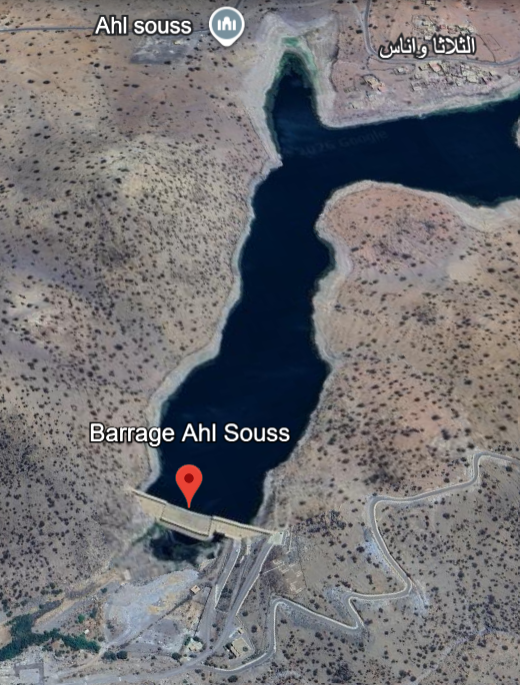
\includegraphics[width=0.55\textwidth]{figures/figure4_location.png}
    \caption{Vue satellitaire du barrage Ahl Souss (A\"it M'zal) sur l'oued Izig, province de Chtouka A\"it Baha. Source : Google Maps (2024).}
    \label{fig:localisation_barrage}
\end{figure}

\section{Caractéristiques hydrologiques}
\label{sec:hydrologie}

Le bassin versant de l'oued Izig présente les caractéristiques physiques suivantes \cite{donnees_hydrologiques, fiche_synoptique} :
\begin{itemize}
    \item Superficie : 187 km²
    \item Altitude moyenne : 1\,287 m
    \item Pluie moyenne annuelle : 269--275 mm
    \item Apport moyen annuel : 5,1 millions de m³ (série de données de 1932 à 2006) \cite{bilans_apports}
    \item Envasement moyen annuel : 100\,000 m³/an
\end{itemize}

Les débits de pointe des crues pour différentes périodes de retour sont \cite{donnees_hydrologiques, fiche_synoptique} :

\begin{table}[H]
    \centering
    \caption{Débits de crues du barrage Ahl Souss}
    \label{tab:debits_crues}
    \begin{tabular}{|c|c|c|}
        \hline
        \textbf{Période de retour (ans)} & \textbf{Débit (m³/s)} & \textbf{Volume (Mm³)} \\
        \hline
        10 & 220 & 2,62 \\
        \hline
        100 & 520 & 6,27 \\
        \hline
        1000 & 820 & 9,85 \\
        \hline
        5000 & 1030 & 12,4 \\
        \hline
    \end{tabular}
\end{table}

L'hydrogramme de crue, supposé triangulaire, présente un temps de base de 7 heures et un temps de montée de 2 heures \cite{donnees_hydrologiques}.

\section{Caractéristiques de la retenue}
\label{sec:retenue}

La retenue du barrage Ahl Souss présente les caractéristiques suivantes \cite{fiche_synoptique, bilans_apports} :
\begin{itemize}
    \item Niveau de retenue normale (RN) : \textbf{600,00 NGM}
    \item Niveau des plus hautes eaux (NPHE) : \textbf{602,86 NGM}
    \item Aire de la retenue au niveau normal : 0,5 km² (50 ha)
    \item Capacité à retenue normale : \textbf{4,76 Mm³}
\end{itemize}

\section{Caractéristiques principales du barrage}
\label{sec:caracteristiques_barrage}

Le barrage Ahl Souss est un ouvrage \textbf{poids en béton compacté au rouleau (BCR)} dont les principales caractéristiques sont \cite{fiche_synoptique, fiche_historique} :
\begin{itemize}
    \item Hauteur maximale sur fondation : 49 m
    \item Hauteur maximale sur terrain naturel : 32,50 m
    \item Longueur en crête : 213,59 m
    \item Largeur en crête : 5 m
    \item Cote de la crête : 604,00 NGM
    \item Fruit du parement amont : \textbf{vertical} (modifié par rapport à l'APD)
    \item Fruit du parement aval : \textbf{0,9 H / 1 V} (modifié)
    \item Volume total de béton : 94\,000 m³ (dont 71\,500 m³ de BCR et 22\,500 m³ de BCV)
\end{itemize}

\section{Description de l'évacuateur de crues}
\label{sec:evacuateur_crues}

L'évacuateur de crues est un ouvrage critique pour la sécurité du barrage, conçu pour transiter les crues exceptionnelles sans endommager l'ouvrage. Ses caractéristiques sont les suivantes \cite{fiche_synoptique, note_calcul_evacuateur} :

\begin{itemize}
    \item \textbf{Type} : Seuil libre en béton de type Creager, implanté dans la partie centrale du barrage.
    \item \textbf{Longueur de déversement} : 70 m.
    \item \textbf{Cote du seuil} : 600,00 NGM (calée au niveau de la retenue normale).
    \item \textbf{Charge maximale sous NPHE} : 2,86 m (calculée après laminage de la crue millénale).
    \item \textbf{Débit évacué sous NPHE} : 730 m³/s.
    \item \textbf{Débit évacué sous NPHEE} : 1\,008 m³/s.
    \item \textbf{Mode de restitution} : Saut de ski.
\end{itemize}

Le profil du seuil, dimensionné pour une charge de 3,20 m, est défini par l'équation \cite{note_calcul_evacuateur} :

\begin{equation}
X^{1,85} = 5{,}376\,Y
\label{eq:profil_creager}
\end{equation}

Le coursier est bordé de murs bajoyers canalisant l'écoulement. La cuillère du saut de ski, calée à la cote \textbf{585,20 NGM}, permet de projeter le jet d'eau loin du pied aval du barrage. Le bec déviateur est tracé selon un arc de cercle de rayon \textbf{3 m} avec un angle de sortie de \textbf{40°} sur l'horizontale \cite{note_calcul_evacuateur}. La distance d'impact du jet est estimée à \textbf{29,5 m} pour la crue de projet.

\section{Description de la vidange de fond}
\label{sec:vidange_fond}

La vidange de fond est un organe essentiel pour la gestion des sédiments et la vidange partielle ou totale de la retenue pour des besoins d'inspection ou de maintenance. Ses caractéristiques sont \cite{fiche_organes_restitution, note_calcul_vidange} :

\begin{itemize}
    \item \textbf{Implantation} : Rive gauche.
    \item \textbf{Type} : Deux conduites en acier indépendantes.
    \item \textbf{Diamètre des conduites} : \textbf{1000 mm} (initialement prévu en 800 mm dans l'APD, modifié en phase d'exécution pour réduire le temps de vidange).
    \item \textbf{Longueur des conduites} : 22,00 m.
    \item \textbf{Cote de calage à l'entrée} : \textbf{585,50 NGM} (ajustée par rapport à la cote 586,00 NGM de l'APD).
    \item \textbf{Volume de retenue correspondant} : 932 788 m³.
    \item \textbf{Capacité sous retenue normale} : \textbf{12 m³/s}.
    \item \textbf{Temps de vidange de la retenue} : \textbf{5 jours}.
    \item \textbf{Équipement hydromécanique} :
    \begin{itemize}
        \item 2 vannes à opercule (papillon) de diamètre 1000 mm par conduite (une vanne de garde et une vanne de réglage), pression nominale 10 Bar.
        \item Une grille métallique de protection de dimensions 1,4 m x 1,4 m.
        \item Commande électrique (moteur 3 kW, 400 V) ou manuelle (volant).
    \end{itemize}
    \item \textbf{Dissipation} : Bassin de dissipation en béton armé de 12 m de longueur, radier à la cote 579,50 NGM, prolongé par un canal en maçonnerie.
\end{itemize}

% SECTION 4.10 : DESCRIPTION DES PRISES D'EAU (AEP ET AGRICOLE)
\section{Description des prises d'eau (AEP et agricole)}
\label{sec:prises_eau}

Le barrage est équipé de plusieurs prises d'eau pour satisfaire les besoins en eau potable et en irrigation \cite{fiche_synoptique, fiche_organes_restitution} :

\begin{itemize}
    \item \textbf{Prises d'eau potable (AEP)} : Trois conduites en acier de diamètre 200 mm, calées à différentes cotes pour permettre un tirage sélectif en fonction de la qualité de l'eau et du niveau de la retenue :
    \begin{itemize}
        \item Cote \textbf{595 NGM}.
        \item Cote \textbf{590 NGM}.
        \item Cote \textbf{586 NGM}.
    \end{itemize}
    Chaque conduite est équipée de vannes de contrôle.
    \item \textbf{Prise agricole} : Une conduite en acier de diamètre 300 mm, calée à la cote \textbf{586,00 NGM}, avec une vanne de contrôle.
\end{itemize}

% SECTION 4.11 : DESCRIPTION DE LA GALERIE D'INJECTION ET DE DRAINAGE
\section{Description de la galerie d'injection et de drainage}
\label{sec:galerie}

Une galerie visiteuse, reliant les deux rives, joue un rôle crucial dans la surveillance et la sécurité de l'ouvrage \cite{fiche_historique, fiche_synoptique} :
\begin{itemize}
    \item \textbf{Fonctions} :
    \begin{itemize}
        \item Permettre l'injection de coulis de ciment pour créer un voile d'étanchéité dans la fondation (injection).
        \item Collecter les eaux de drainage pour mesurer et contrôler les sous-pressions (drainage).
        \item Servir d'accès pour l'inspection et l'auscultation de l'intérieur du barrage.
    \end{itemize}
    \item \textbf{Caractéristiques} : La galerie a été surélevée à la cote \textbf{573,50 NGM} en phase d'exécution (contre 570 NGM à l'APD) pour éviter les risques d'inondation. Sa largeur a été portée à \textbf{3 m} pour faciliter les travaux de forage.
\end{itemize}

% SECTION 4.12 : DESCRIPTION DE LA DÉRIVATION PROVISOIRE
\section{Description de la dérivation provisoire}
\label{sec:derivation_provisoire}

Pendant la construction, il a fallu dévier l'oued pour travailler à sec \cite{fiche_historique, fiche_synoptique} :
\begin{itemize}
    \item \textbf{Type} : Deux pertuis bétonnés disposés en rive gauche, traversant provisoirement le corps du barrage.
    \item \textbf{Dimensions des pertuis} : 2 x 4,50 m de large x 5,00 m de haut.
    \item \textbf{Crue de chantier} : Dimensionnée pour la crue vingtenale (Q20 = 310 m³/s).
\end{itemize}

% SECTION 4.13 : ASPECTS PARTICULIERS ET ADAPTATIONS EN COURS DE CHANTIER
\section{Aspects particuliers et adaptations en cours de chantier}
\label{sec:adaptations_chantier}

Plusieurs adaptations ont été apportées au projet initial (APD) durant la phase d'exécution pour s'adapter aux conditions réelles du site ou pour optimiser l'ouvrage \cite{fiche_historique, note_geologique_2003} :

\begin{itemize}
    \item \textbf{Décalage de l'axe du barrage} : L'axe définitif a été décalé d'une trentaine de mètres en aval suite aux prospections géologiques qui ont révélé du rocher altéré sur la rive gauche.
    \item \textbf{Modification du profil du barrage} : Le profil est passé d'un parement amont penté (0,2H/1V) à un parement amont \textbf{vertical}, et le parement aval de 0,8H/1V à \textbf{0,9H/1V}. La largeur en crête est passée de 3 m à \textbf{5 m}, et sa cote de 603,50 à \textbf{604,00 NGM}.
    \item \textbf{Approfondissement des fouilles} : La découverte d'une zone de rocher très altéré en fond de vallée (épaisseur de 7 à 8 m) a nécessité un approfondissement des fouilles de 7 à 9 m, avec des cotes de fondation finales à 555 NGM (amont) et 556 NGM (aval).
    \item \textbf{Élargissement du diamètre des conduites de vidange} : Le diamètre est passé de 800 mm à \textbf{1000 mm}, réduisant le temps de vidange de la retenue d'environ 64 \%.
    \item \textbf{Surélévation de la galerie d'injection} : La galerie a été surélevée de la cote 570 NGM à \textbf{573,50 NGM} pour éviter les risques d'inondation.
    \item \textbf{Substitution du BCR par du BCV pour le couronnement} : Le BCR prévu pour le couronnement (cotes 598,45 à 604,00 NGM) a été remplacé par du BCV en raison de l'espace de travail trop restreint pour les engins de compactage.
\end{itemize}

% SECTION 4.14 : CONCLUSION
\section{Conclusion}
\label{sec:conclusion_chap4}

Le barrage Ahl Souss constitue un ouvrage hydraulique complexe, dont la conception a intégré des innovations technologiques comme le béton compacté au rouleau, et a su s'adapter aux contraintes géologiques et opérationnelles rencontrées en cours de chantier. La description détaillée de ses caractéristiques et de ses organes annexes, notamment l'évacuateur de crues et la vidange de fond, pose les bases nécessaires à la modélisation numérique qui fera l'objet de la suite de ce rapport.
